%%---------------------------------------------------------------------------%%
%%------------ 第二章:预备知识 -----------------------------------%%
%%---------------------------------------------------------------------------%%


\chapter{预备知识}
\label{chapter:mixed-element}


我们把后文中用到的混合有限元方法和构建混合元所用的几何遗传树结构,以及移动网格方法,
在本章中做简要描述和历史回顾。
\section{混合有限元}
    混合有限元方法的专著可以参考F.Brezzi和M.Fortin \cite{brezzi2012mixed}。二阶
    椭圆性问题的混合有限元方法就是基于Hellinger-Reissner变分原理的有限元方法。在
    流体中混合元方法是把速度和压力耦合在一起求解,因而精度得到提高,体现出相对于
    分开求解速度和压力有限元方法的优势。另外,对于不可压流体中的Galenkin逼近,只能
    采取混合有限元。在这一节中,我们以Stokes方程为例,来介绍混合元方法。Stokes方
    程可以看做是Navier-stokes的简化,去掉了非线性项。Stokes方程有两个需要求解的函数速
    度$\vec{u}$和压力$p$是耦合的,并且速度要满足质量守恒的条件($\nabla \cdot \vec{u} = 0$)。
    因此,需要我们用混合有限元方法来求解方程。为确保方程的解存在唯一,速度
    和压力所在的有限元空间必须满足inf-sup条件。如果有限元不满足inf-sup(LBB)
    条件,例如在四边形单元中的$Q_1-Q_1$,$Q_1-P_0$,三角形单元中的$P_1-P_1$,$P_1-P_0$元,
    还需要在压力空间上做稳定化。

    下面我们以Stokes方程为例,给出它的混合变分形式。Stokes方程可以表示为:
    \begin{equation}
        \begin{aligned}
            -\bigtriangleup \vec{u} + \nabla p = f \quad \text{在}\Omega \text{内}, \\
            \nabla \cdot \vec{u} = 0 \quad \text{在}\Omega \text{内},\\
            \vec{u} = 0 \qquad \text{在}\partial \Omega \text{上},
        \end{aligned}
        \label{eq::stokes}
    \end{equation}
    令
    \begin{eqnarray}
        a(\vec{u},\vec{v}) = \int_{\Omega} \nabla \vec{u} \cdot \nabla \vec{v},  \\
        b(\vec{u}, q) = -\int_{\Omega} \nabla \cdot \vec{u} q.
    \end{eqnarray}
    为简便起见,我们这里只考虑二维情形。对(\ref{eq::stokes})利用格林公式,可以得到混合变分
    形式:寻找$(\vec{u}, p) \in (H_0^1(\Omega))^2 \times L_0^2(\Omega)$ 使得
    \begin{equation}
        \begin{aligned}
            a(\vec{u}, \vec{v}) + b(\vec{v}, p) &=& (f,v), \\
            b(\vec{u},q) &=& 0.
        \end{aligned}
        \label{eq::weak_form_stokes}
    \end{equation}
    对$\forall (\vec{v}, q) \in X \times P, X \in (H_0^1(\Omega))^2, P \in
    (L_0^2)$, $L_0^2 = \{q \in L^2(\Omega)| \int_{\omega}q dx = 0$。其中有限元空间
    $X,P$要满足inf-sup条件或者LBB条件,即
    \begin{equation}
        \beta ||q||_{P} \leq \sup\limits_{\vec{v} \in X}\frac{b(v, q)}{||\vec{v}||_X},
        \quad \forall q \in P.
        \label{eq::LBB_cond}
    \end{equation}
    这个条件的验证由很多专著中给出,例如(\cite{brezzi2012mixed},\cite{brenner2007mathematical},
    \cite{cuvelier1986finite}等)。我们不加证明地给出如下定理:
    \begin{theorem}
        问题(\ref{eq::weak_form_stokes})的解存在唯一。
    \end{theorem}
    在研究用混合元去离散Stokes问题时,我们构造的有限维子空间$(X_h, P_h) \subset (X, P)$要满足离散的
    inf-sup条件:
    \begin{equation}
        \beta_0||q_h||_{P_h} \leq \sup\limits_{\vec{v}_h \in X_h}\frac{b(\vec{v}_h, q_h)}{||\vec{v}_h||_{X_h}},
        \quad \forall q_h \in P_h.
        \label{eq::discretized_LBB_cond}
    \end{equation}
    其中$\beta_0$是一个跟网格尺度无关的常量。Mini元,RT元以及Taylor-Hood元都是满足离散的LBB条件的。
    我们得到(\ref{eq::weak_form_stokes})对应的离散形式:寻找$(\vec{u}_h, p_h) \in X_h \times P_h$ 使得
    \begin{equation}
        \begin{aligned}
            a(\vec{u}_h, \vec{v}_h) + b(\vec{v}_h, p_h) &=& (f_h,v_h), \\
            b(\vec{u}_h, q_h) &=& 0.
        \end{aligned}
        \label{eq::discreted_weak_form_stokes}
    \end{equation}
    求解(\ref{eq::discreted_weak_form_stokes}),得到的离散数值解$(\vec{u}_h, p_h)$, 如果$(\vec{u}, p)$
    是弱形式(\ref{eq::weak_form_stokes})的解,则我们可以得到对应的误差估计:
    \begin{equation}
        ||\vec{u} - \vec{u}_h||_1 + ||p - p_h||_0 \leq C\{\inf\limits_{\vec{v}_h \in X_h} ||\vec{u} - \vec{v}_h||_1
        + \inf\limits_{q_h \in P_h} ||p - q_h||_0\}.
    \end{equation}

    我们倾向于使用满足LBB条件的混合元Taylor-Hood元,如$P_2-P_1$,$Q_2-Q_1$元,即速度
    是二次元,压力是线性元。在实际的工程计算中,因为线性元简单,所以比较受欢迎。因此
    我们设想,如果把稳定的Taylor-Hood元中的速度二次元换成线性元,同时又要保证速度和
    压力满足inf-sup条件,这就是$P_1isoP_2P_1$的想法。如图\ref{fig::p-v}所示,因为压力
    是线性元,因此在一个三角形单元上有三个自由度,分布在三角形的三个顶点上。同样地,
    速度是二次元,在这个三角形单元个有6个自由度,分布在三角形的三个顶点和三边的中点
    上。如果这个三角形单元加密一次,即连接三边中点,因此得到四个小三角形。这样在每个
    小三角形上有分布着三个自由度。在\cite{bercovier1979error}中证明了$P_1isoP_2P_1$是
    满足inf-sup条件的。令$X_h = X_{h/2}^1, P_h = P_h^1$,则
    \begin{theorem}
        如果$\Omega$是一个多边形, 并且对所有$h$都有$\Omega_h = \Omega$,如果$\Omega_h$中所有的三角形都至少有一个顶点
        不在$\Omega$的边界$\Gamma$上, $X_h, P_h$是满足LBB条件的, 那么问题(\ref{eq::discreted_weak_form_stokes})
        是有唯一解$(\vec{u}_h, p_h) \in X_h \times (P_h/R)$($p_h$除了一个常数外是确定的)。
    \end{theorem}
    定理的过程我们不再给出,\cite{bercovier1979error}中还给出了$P_1isoP_2P_1$元的误差估计:
    \begin{eqnarray}
        {|\nabla (\vec{u} - \vec{u}_h)|}_0 \leq h K( ||\vec{u}||_{(H^2(\Omega))^2} + ||p||_{H^1(\Omega)/R}), \\
        {|\nabla (p - p_h)|}_0 \leq K (||\vec{u}||_{(H^2(\Omega))^2} + ||p||_{H^1(\Omega)/R} ).
    \end{eqnarray}

    但是需要注意到图\ref{fig::p-v}中,每个小三角形上的三个自由度,其实是大的三角形6个自由
    度中的3个。因此,在做速度单元和压力单元拼装的时候,需要先找到速度单元基函数所在的大单
    元,然后用大单元的基函数中正好位于当前速度单元上基函数与压力单元上的基函数进行拼装。
    这会带来一些技术上的困难。如果图\ref{fig::p-v}右中每个小三角形上的自由度都是局部在一个单元
    上,这时跟$P_1isoP_2P_1$拥有同样的网格结构,也满足inf-sup条件,但速度单元全部是
    线性元,因此称作$4P1-P1$元。在这种情况下,只要建立速度单元和压力单元之间的索引,
    速度单元与压力单元间的拼装变得容易很多。这时速度和压力分别在两套网格上,其中速度
    网格由压力网格加密一次得到。

    \begin{figure}
      \centering
      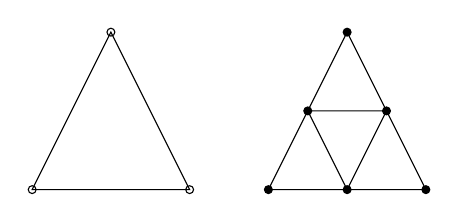
\begin{tikzpicture}
        % 三角形
        \draw (2, 1) -- (4, 1) -- (3, 3) -- cycle;
        % 三个顶点
        \draw (2, 1) circle(0.05cm);
        \draw (4, 1) circle(0.05cm);
        \draw (3, 3) circle(0.05cm);
        % 四个三角形
        \draw (5, 1) -- (6, 3) -- (7, 1) -- cycle;
        \draw (5.5, 2) -- (6.5, 2) -- (6, 1) -- cycle;
        % 六个顶点
        \draw [fill = black] (5, 1) circle(0.05cm);
        \draw [fill = black] (6, 3) circle(0.05cm);
        \draw [fill = black] (7, 1) circle(0.05cm);
        \draw [fill = black] (5.5, 2) circle(0.05cm);
        \draw [fill = black] (6.5, 2) circle(0.05cm);
        \draw [fill = black] (6, 1) circle(0.05cm);
      \end{tikzpicture}
      \caption{左: 压力 $p$ 单元, $\circ$ 为$p$单元上的自由度;
               右: 4个速度$v$ 单元, $\bullet$ 表示$v$单元上的自由度.}
      \label{fig::p-v}
    \end{figure}

\section{几何遗传树结构}
    在上一节中,我们提到速度单元和压力单元之间的索引,而这个索引的建立利用了\cite{li2005multi}
    中的几何遗传树结构。这种树结构是用来做h-自适应,下面我们就介绍一下这种树结构。

    在h-自适应中,两个耦合在一起的物理量(如上一节提到的速度$u$和压力$p$),有可能在不同的地方出现奇异,
    因此需要分别在两套网格上离散数值解。在拼装$\int_{\Omega} \nabla \cdot \vec{u} p$这一项时,因为$\vec{u}$
    和$p$在不同的网格上,因此需要构建两套网格之间的联系。如果函数在相对于计算区域来说,很小的区域内有奇异,
    好的网格需要在这个奇异出现的地方网格非常集中。特别地,如果最小的网格单元和最大的网格单元面积相差上百倍,
    这时候建立两个网格之间对应的代价是非常昂贵的。为了创建高效的多网格自适应策略,\cite{li2005multi}中选取
    了几何遗传树,具有遗传性的网格结构可以描述为点、线、面、体。并且针对无结构网格,加密也是通过按层次来加密的。
    这种分层的数据结构可以提供简单的编程方法和快速的网格加密算法,以及多重网格求解器。

    我们以二维区域$\Omega$上的一个三角剖分$\mathcal{T}_0$为例,来介绍一下几何遗传树结构。为与有限元空间的单元
    区分开,称三角剖分中的单元为几何单元。$\tau$为$\mathcal{T}_0$的几何单元。三角剖分中所有几何性质都有属于的
    关系,即如果一条边是一个三角形三边中的一条,则称这条边属于这个三角形。同样的,如果一个点是一条边两个顶点
    中的一个,则称这个点属于这条边。三角剖分中的一个三角形可以被加密成四个小的三角形。在三角形加密的过程中,三
    条边分别被分成了两部分。当三角剖分中所有的三角形都加密一次,我们可以得到一个更密的三角剖分$\mathcal{T}_1$,
    这就是$\mathcal{T}_0$的一次全局加密。经过逐次加密,我们可以得到一系列的三角剖分$\{ \mathcal{T}_n\}$。 如果
    $\mathcal{T}_n$中的一个三角形$\tau_1$位于$\mathcal{T}_{n-1}$中的三角形$\tau_0$中,则$\tau_1$被称作是$\tau_0$
    的一个孩子。我们给$\mathcal{T}_0$中的所有三角形一个虚拟的父亲,与所有从$\mathcal{T}_0$的三角形中派生出的所有
    四叉树组成了一个树的数据结构,如图\ref{fig::hgrometrytree}所示。这颗树也被称为几何遗传树。
    \begin{figure}[h]
        \begin{minipage}[t]{0.4\textwidth}
          \centering
          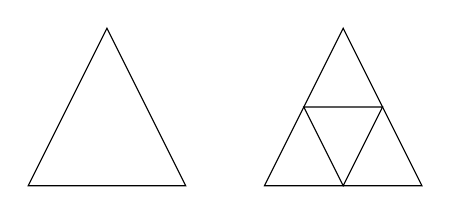
\begin{tikzpicture}
            % 三角形
            \draw (2, 1) -- (4, 1) -- (3, 3) -- cycle;
            \draw (5, 1) -- (6, 3) -- (7, 1) -- cycle;
            \draw (5.5, 2) -- (6.5, 2) -- (6, 1) -- cycle;
          \end{tikzpicture}
          \caption{全局加密一次的网格}
        \end{minipage}
        \begin{minipage}[t]{0.6\textwidth}
          \centering
          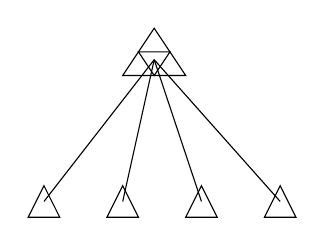
\begin{tikzpicture}
            %五个小三角形
            \draw (1.0, 0.0) -- (1.2, 0.4) -- (1.4, 0.0) -- cycle;
            \draw (2.0, 0.0) -- (2.2, 0.4) -- (2.4, 0.0) -- cycle;
            \draw (3.0, 0.0) -- (3.2, 0.4) -- (3.4, 0.0) -- cycle;
            \draw (4.0, 0.0) -- (4.2, 0.4) -- (4.4, 0.0) -- cycle;
            \draw (2.6, 2.4) -- (2.2, 1.8) -- (3.0, 1.8) -- cycle;
            \draw (2.4, 2.1) -- (2.6, 1.8) -- (2.8, 2.1) -- cycle;
            %四条线
            \draw (2.6, 2.0) -- (1.2, 0.2);
            \draw (2.6, 2.0) -- (2.2, 0.2);
            \draw (2.6, 2.0) -- (3.2, 0.2);
            \draw (2.6, 2.0) -- (4.2, 0.2);
          \end{tikzpicture}
          \caption{它的几何遗传树}
        \end{minipage}
      \caption{几何遗传树结构}
      \label{fig::hgrometrytree}
    \end{figure}
    用几何遗传树结构来构建h-自适应的内容就不再详细介绍了。

\section{移动网格方法}
    移动网格方法常常用在数值计算中,寻找好的网格(跟具体问题有关),并在
    网格上进行数值求解,使得在不增加自由度的前提下,尽可能的提高计算精
    度。移动网格方法包括网格的移动策略,以及在方程在网格上的数值求解算
    法。在\cite{budd2009adaptivity}、\cite{huang2011book}、\cite{tang2007book}
    中系统地给出了移动网格方法的介绍。移动网格的策略是基于等分布原则
    (Equi-distribute Principle),这是de Boor在1974年\cite{boor1974goodII}
    提出的。等分布原则是根据一个能反映局部网格计算质量的指标,比如误差,
    移动网格节点使得这个指标在网格上均匀分布。如果在计算结果误差比较大的
    地方网格集中,尽量使得误差分布的比较均匀,从而提高计算精度。

    一些符号的定义如下:令$\Omega \subset \mathbb{R}^N, N = 1, 2, 3$代表
    物理区域,$\vec{x}$代表物理区域上的坐标。同样地,$\Omega_c \subset
    \mathbb{R}^N$表示逻辑区域(或称计算区域),$\vec{\xi}$为其坐标。

        de Boor 给出了一维情形的证明,如下:

    假设$\Omega = [a, b]$,$\Omega_c = [0, 1]$分别为物理区域和计算区域,
    在$\Omega_c$上有一个均匀网格$\{\xi_j = \frac{j}{N}| j = 0, 1, \cdots, N\}$,



\section{预处理方法}
    我们将分别对Stokes方程和Navier-Stokes方程,介绍预处理的方法。
    \subsection{针对Stokes方程}
        我们通过选取有限元空间基函数对\eqref{eq::weak_form_stokes}进行离散,可以得到一个线性方程租,我们定义这个线性方程组的
        系数矩阵为:
        \begin{equation}
            K = \left[
                \begin{array}{ll}
                 \vec{A} & B^T\\
                 B & -C
                \end{array}
                \right]
        \end{equation}
        其中如果用满足LBB条件的混合元做近似,则 $C = 0$。因为本文中我们选取的是满足LBB条件的$4P1-P1$元,所以我们下面均考虑 $C = 0$ 的情形。令 $\vec{v}_h \in X_h$ 和 $q_h \in P_h$,$X_h$ 和 $P_h$ 是在第一节中提到的有限元空间。我们先来定义 $\vec{v}_h, q_h$ 的范数:
        \begin{align}
            ||\nabla \vec{v}_h|| := <\vec{A}\vec{v}, \vec{v}>^{1/2}, \\
            ||q_h|| := <Qq, q>^{1/2}.
            \label{eq::norm}
        \end{align}
        其中$\vec{v}$ 和 $\vec{q}$ 是速度和压力变量在基函数$\{\vec{\phi}_j \}_{j = 1}^{n_u}$ 和 $\{\vec{\psi}_k \}_{k = 1}^{n_p}$ 下的系数。这里的 $\vec{A}$ 是离散的向量形式的刚度矩阵:
        \begin{eqnarray}
            \vec{A} = [a_{ij}], \quad a_ij = \int_\Omega \nabla \vec{\phi}_i : \nabla \vec{\phi}_j, \qquad i,j = 1, \cdots, n_u
        \end{eqnarray}
        并且 $Q$ 是压力质量矩阵:
        \begin{equation}
            Q = [q_{kl}],\quad q_{kl} = \int_\Omega \psi_k \psi_l, \qquad k,l = 1, \cdots, n_p.
        \end{equation}
        我们用标准的分量形式的向量基函数,在二维问题情形中
        \begin{equation}
            <\vec{A}\vec{v}, \vec{v}> \equiv <A\vec{v}_x, \vec{v}_x> + <A\vec{v}_y, \vec{v}_y>,
        \end{equation}
        其中 $A$ 是 $n \times n$ 的拉普拉斯矩阵。
        我们称矩阵 $B \vec{A}^{-1} B^T$ 为压力Schur补。我们考虑$Q^{-1}B\vec{A}^{-1}B^T$ 的特征值的范围。我们先考虑边界全部是Dirichlet边界的流体问题,我们先给出一些定义。
        \begin{definition}
            \label{def::min_angle_cond}对于一系列的三角网格$\{\mathcal{T}_h\}$,如果存在一个最小的角度
            $\theta_* > 0$,使得$\mathcal{T}_h$中的所有单元满足$\theta_{T} > \theta_*$,那么$\mathcal{T}_h$称作是形正则的。
        \end{definition}
        \begin{proposition}
            \label{pro::bound_mass} 对于$\mathbb{R}^2$ 空间中的具有形正则性质的一个剖分,$\vec{P}_1$是建立在这个剖分上的一个近似,那么质量矩阵$Q$以如下的形式近似
            数量单位矩阵:
            \begin{equation}
                c\uline{h}^2 \leq \frac{<Q\vec{v}, \vec{v}>}{<\vec{v}, \vec{v}>} \leq Ch^2
                \label{eq::bound_mass}
            \end{equation}
            对所有的$\vec{v} \in \mathbb{R}^n$。这里$\uline{h} = \min_{\bigtriangleup_k \in \mathcal{T}_h} h_k$ 并且 $h = \max_{\bigtriangleup_k \in \mathcal{T}_h} h_k$。常数$c$ 和 $C$ 都是跟$\uline{h}$ 和 $h$ 无关的。
        \end{proposition}

        \begin{definition}[拟一致剖分]
            \label{theo_quasi_uni_subd}对于一系列的三角网格$\{\mathcal{T}_h\}$,如果存在着一个常读$\rho > 0$ 使得对于$\{\mathcal{T}_h\}$中的每一个网格,都有 $\uline{h} \geq \rho h$,那么我们就称 $\{\mathcal{T}_h\}$ 是拟一致的。
        \end{definition}

        对于$\mathcal{R}^2$空间的一个拟一致剖分,并且它的单元都是形正则的,那么界限 \eqref{eq::bound_mass} 可以简化为:
        \begin{equation}
            c h^2 \leq \frac{<Q \vec{v}, \vec{v}>}{<\vec{v}, \vec{v}>} \leq C h^2 \quad \mbox{对所有的} \vec{v} \in \mathbb{R}^n.
            \label{eq::bound_mass_simpify}
        \end{equation}
        \eqref{eq::bound_mass_simpify} 是跟空间的维数有关的。对于 $\mathbb{R}^3$ 中的一个区域,进行拟一致剖分,则这个剖分上的所有四面体单元,对应有界:
        \begin{equation}
            c h^3 \leq \frac{<Q \vec{v}, \vec{v}>}{<\vec{v}, \vec{v}>} \leq C h^3 \quad \mbox{对所有的} \vec{v} \in \mathbb{R}^n.
            \label{eq::bound_mass_R3}
        \end{equation}

        \begin{remark}
            如果剖分是拟一致的,那么对于任意近似$\vec{P}_m, \vec{Q}_m, m \geq 2$,有界性 \eqref{eq::bound_mass_simpify} 都成立,但是 $c$ 和 $C$ 都跟 $m$ 有关。
        \end{remark}

        \begin{theorem}
            \label{theo_mass_spectrual_eq} 对于 $\partial \Omega = \partial \Omega_D$ 的流体问题,用满足LBB的混合元近似并且 $\mathbb{R}^2$上的拟一致的剖分是形正则的,则
            压力Schur补矩阵$B \vec{A}^{-1} B^T$ 谱等价于压力质量矩阵$Q$:
            \begin{equation}
                \gamma^2 \leq \frac{(B \vec{A}^{-1} B^T \vec{q}, \vec{q})}{Q\vec{q},\vec{q}} \quad \mbox{对所有的} \vec{q} \in \mathbb{R}^{n_p} \mbox{使得} \vec{q} \neq \vec{1}.
                \label{eq::lower_uper_bound}
            \end{equation}
            inf-sup 常量$\gamma$ 被限制在$0$以外,并且跟网格尺度$h$无关。并且有效的条件数满足
            \begin{equation}
                \kappa(B\vec{A}^{-1}B^T) \leq C/(c\gamma^2),
            \end{equation}
            其中$c$ 和 $C$ 是\eqref{eq::bound_mass_simpify}中的常数。
        \end{theorem}

        \begin{proof}
            我们先来证明下界。离散inf-sup稳定性条件的代数表示:
            \begin{equation}
                \gamma \leq \min_{q_h \neq \mbox{constant}} \max_{\vec{v}_h \neq \vec{0}} \frac{|(q_h, \nabla \cdot \vec{v}_h)|}{||\nabla \vec{v}_h|| ||q_h||}.
            \end{equation}
            特别的,运用\eqref{eq::norm}中的矩阵范数,并且有$|(q_h, \nabla \cdot \vec{v}_h)| = (q, B\vec{v})$, 我们有:
            \begin{align}
                \gamma & \leq  \min_{\vec{q} \neq \vec{1}} \max_{\vec{v} \neq \vec{0}} \frac{|<q, B\vec{v}>|}{<\vec{A}\vec{v}, \vec{v}>^{1/2} <Q\vec{q}, \vec{q}>^{1/2}} &\\  \notag
                & =  \min_{\vec{q} \neq \vec{1}} \frac{1}{<Q\vec{q}, \vec{q}>^{1/2}} \max_{\vec{w} = \vec{A}^{1/2}\vec{v} \neq \vec{0}} \frac{|<\vec{q}, B \vec{A}^{-1/2} \vec{w}>|}{<\vec{w}, \vec{w}^{1/2}>} &\\ \notag
                & =  \min_{\vec{q} \neq \vec{1}} \frac{1}{<Q\vec{q}, \vec{q}>^{1/2}} \max_{\vec{w} \neq \vec{0}} \frac{|<\vec{A}^{-1/2}B^Tq, \vec{w}>|}{<\vec{w}, \vec{w}>^{1/2}} &\\ \notag
                & =  \min_{\vec{q} \neq \vec{1}} \frac{<\vec{A}^{-1/2}B^Tq, \vec{A}^{-1/2}B^Tq>^{1/2}}{<Q\vec{q}, \vec{q}>^{1/2}} &\\ \notag
                & = \min_{\vec{q} \neq \vec{1}} \frac{<B \vec{A}^{-1}B^T\vec{q}, \vec{q}>}{<Q\vec{q}, \vec{q}>^{1/2}}& \notag
            \end{align}
            因为它的极大值在$\vec{w} = \pm \vec{A}^{-1/2}B^T \vec{q}$。因此,我们可以看到
            \begin{equation}
                \gamma^2 = \min_{\vec{q} \neq \vec{1}} \frac{<B\vec{A}^{-1}B^T \vec{q}, \vec{q}>}{<Q\vec{q}, \vec{q}>},
                \label{eq::lower_bound}
            \end{equation}
            则下界得证。
            现在我们来证明上界,上界是由微分算子的性质得到的。首先,应用cauchy-Schwarz不等式,我们有
            \begin{equation}
                |(q_h, \nabla \cdot \vec{v}_h)| \leq ||q_h|| ||\nabla \cdot \vec{v}_h||.
                \label{eq::cauchy_schwarz_inequality}
            \end{equation}
            第二,注意到 $\vec{v}_h \in \mathcal{H}_0^1$(因为$\partial \Omega  = \partial \Omega_D$),将 $\vec{v}_h$ 带入到下列等式中:
            \begin{equation}
                \int){\Omega} \nabla \vec{w} : \vec{v} \equiv \int_{\Omega} (\nabla \cdot \vec{w})(\nabla \vec{v}) + \int_{\Omega} (\nabla \times \vec{w}) : (\nabla \times \vec{v}),
            \end{equation}
            其中这个等式是对任意属于Sobolev空间
            \begin{equation}
                \mathcal{H}_0^1 = \{ \vec{u} \in \mathcal{H}^1(\Omega) | \vec{u} = \vec{0} \mbox{在} \partial \Omega \mbox{上} \},
            \end{equation}
            中的任意函数$\vec{w}, \vec{v}$ 都成立的,因此我们有
            \begin{equation}
                ||\nabla \vec{v}_h||^2 = ||\nabla \vec{v}_h||^2 + ||\nabla \times \vec{v}_h||^2 \geq ||\nabla \vec{v}_h||^2.
                \label{eq::identiy_v_h}
            \end{equation}
            最后,结合 \eqref{eq::cauchy_schwarz_inequality} 和 \eqref{eq::identiy_v_h},我们得到
            \begin{equation}
                \frac{|(q_h, \nabla \cdot \vec{v}_h)|}{||\nabla \vec{v}_h|| ||q_h||} \leq 1.
            \end{equation}
            将上式展开成矩阵形式,如推导 \eqref{eq::lower_bound} 中类似,可以得到 \eqref{eq::lower_uper_bound} 中的上界。
            运用 \eqref{eq::bound_mass} 中的质量矩阵条件数的有界性,我们可以得到 Schur 补矩阵的条件数有界
            \begin{equation}
                \gamma^2 \frac{<Q\vec{q}, \vec{q}>}{<\vec{q}, \vec{q}>} \leq \frac{<B \vec{A}^{-1}B^T \vec{q}, \vec{q}>}{\vec{q}, \vec{q}} \leq \frac{<Q \vec{q}, \vec{q}>}{\vec{q}, \vec{q}}
            \end{equation}
        \end{proof}

        \begin{remark}
            在 $\mathbb{R}^3$ 中的拟一致剖分上的四面体单元,如果是稳定的混合元近似,那么Schur
            补矩阵的有界性同样成立。质量矩阵的有界性由 \ref{eq::bound_mass_R3} 中给出。
        \end{remark}

        同样地,对于边界中包含 Neumann 条件的流体问题,特征值的界在命题 \ref{pro::schur_bound_neumann} 中给出。

        \begin{proposition}
            \label{pro::schur_bound_neumann}对任意 $\int_{\partial \Omega_N} ds \neq 0$ 的流体问题,用一个一致稳定混合元近似去离散,并且这个有限元近似是建立在 $\mathbb{R}^2$ 上的一个形正则、拟一致的剖分上,那么压力Schur补矩阵满足
            \begin{equation}
                \gamma_N^2 \leq \frac{<B\vec{A}B^T \vec{q}, \vec{q}>}{<Q\vec{q}, \vec{q}>} \leq 2 \quad \mbox{对所有的 } \vec{q} \in \mathbb{R}^{n_p}.
            \end{equation}
            常数 $\gamma_N$ 是不为$0$的有界常数,并且跟网格尺度 $h$ 无关。
        \end{proposition}
        对于 $P_2-P_1, Q_2-Q_1$ 混合元近似,是满足inf-sup条件的,即存在一个不为 $0$ 的inf-sup常量 $\delta$,使得
        \begin{equation}
            \delta \leq \min_{q_h \neq \mbox{constant}} \max_{\vec{v}_h \neq \vec{0}} \frac{|(q_h, \nabla \cdot \vec{v}_h)|}{||\vec{v}_h|| ||\nabla q_h||}.
            \label{eq::inf_sup_p2p1}
        \end{equation}
        我们是在 $L^(\Omega)$ 空间中估计速度,在 $\mathcal{H}^1{\Omega}$ 中估计压力,这跟一般的inf-sup条件有些相反。我们先来定义速度质量矩阵 $\heiti{Q}$,
        \begin{equation}
            \heiti{Q} = [\heti{q}_{ij}], \quad \heiti{q}_{ij} = \int_{\Omega} \vec{\phi}_i \cdot \vec{\phi}_j, \qquad i,j = 1, \cdots, n_u,
        \end{equation}
        和压力的刚度矩阵 $A_p$,
        \begin{equation}
            A_p = [a_{kl}], \quad a_{jl} = \int_{\Omega} \nabla \psi_k \cdot \psi_l, \qquad i,j = 1, \cdots, n_p.
        \end{equation}
        那么按照 \eqref{eq::lower_bound} 的推导,则 \eqref{eq::inf_sup_p2p1} 可以重新写为
        \begin{equation}
            \delta^2 = \min_{\vec{q} \neq \vec{1}} \frac{<B \heiti{Q}^{-1} B^T \vec{q}, \vec{q}>}{<A_p\vec {q}, \vec{q}>}.
        \end{equation}
        矩阵$B \heiti{Q}^{-1} B^T$ 通常被叫做一致压力泊松矩阵,详见 \cite{gresho1998incompressible}。对于封闭流体的边界条件,这个矩阵是奇异的,其他情况下,是
        不奇异的。计算 $P_1-P_1$ 近似的最大最小特征值,我们发现在均匀网格上,并且对封闭流体的边界条件,有
        \begin{equation}
            \frac{1}{2} < \frac{<B \heiti{Q}^{-1} B^T \vec{q}, \vec{q}>}{<A_p \vec{q}, \vec{q}>} \leq 1 \quad \mbox{对所有的 } \vec{q} \in \mathbb{R}^{n_p}, \vec{q} \neq \vec{1}.
        \end{equation}

\begin{figure}[h!]
\centering
\subfigure[]{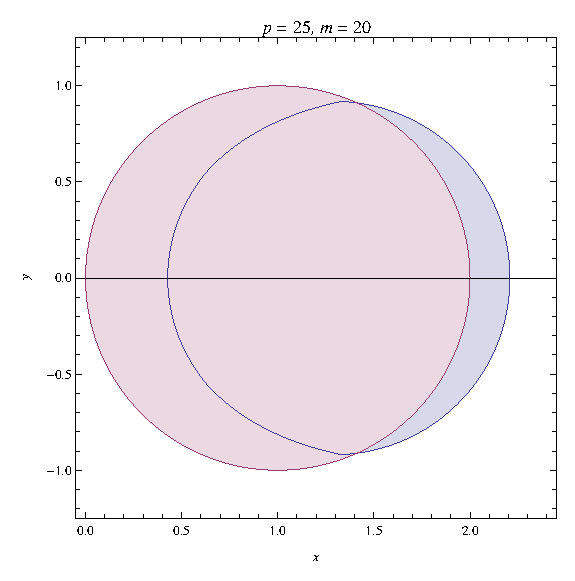
\includegraphics[width=0.3\textwidth]{fig_NM_ConvReg_p25m20.eps}}

\caption{由~(\ref{set:R_NM})~给出的~$\MCR_1$~在九种不同情形~($p$~分别取~25,
100, 400~及~$m$~分别取~20, 100, 500)~下的近似域,
其中红色域表示集合~$\{z\in\CS: 1-z \in \overline{\MCD}_1\}$},
而蓝色域表示集合~$\{z\in \CS: 1-z \in \MCD_{0,1}
\bigcap\MCD_{2,1}\}.$\label{fig:NM_ConvReg}
\end{figure}




\section{预备引理}










\begin{algorithm}
\floatname{algorithm}{算法}
\caption{Preprocessing iterative
framework for computing $A^{1/p}$} \label{al:SIM} Given $A \in
\CS^{n \times n}$ with no nonpositive real eigenvalues, an integer
$p = 2^{k_0}q$ with $k_0 \geq 0$ and $q$ odd. This algorithm
computes the principal $p$th root of matrix $A$ via a Schur
decomposition and some iterative method.
%\newcounter{newlist}
\begin{list}{\arabic{newlist}.}{\usecounter{newlist}
\setlength{\rightmargin}{0em}\setlength{\leftmargin}{1.2em}}
\item
Compute the Schur decomposition of $A = QRQ^*$;
\item
If $q = 1$, then $k_1 = k_0$; else choose the smallest $k_1 \geq
k_0$ such that for each eigenvalue $\lambda$ of matrix $A$,
$\lambda^{1/2^{k_1}}$ belongs to some region $\MCR$;
\item
Compute $B = R^{1/2^{k_1}}$ by taking the square root $k_1$ times;
if $q = 1$, then set $X = QB\tran{Q}$; else continue;
\item
Compute $C = B^{1/q}$ by using some iterative method and set $X = Q
C^{2^{k_1 - k_0}} \tran{Q}$.
\end{list}
\end{algorithm}



\begin{figure}[h!]
\centering
\subfigure[]{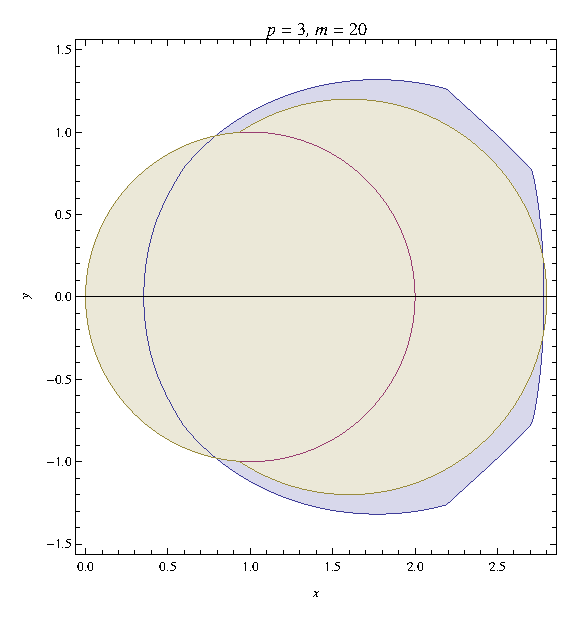
\includegraphics[width=0.3\textwidth]{fig_NM_PraConvReg_p3m20.eps}}

\end{figure}





